\documentclass[12pt,a4paper]{article}
\usepackage[margin=2.5cm]{geometry}
\usepackage{tikz}
\usetikzlibrary{shapes.geometric, positioning, calc, arrows.meta}
\usepackage{float}
\usepackage{tabularx}
\usepackage{booktabs}
\usepackage{colortbl}
\usepackage{amsmath}
\usepackage{amssymb}
\usepackage{enumitem}
\usepackage{hyperref}
\usepackage{fancyhdr}
\setlength{\headheight}{15pt}
\usepackage[dvipsnames,table]{xcolor}
\usepackage{tcolorbox}
\tcbuselibrary{skins, breakable}
\usepackage{titlesec}

% Section styling
\titleformat{\section}{\color{Maroon}\Large\bfseries}{\thesection}{1em}{}[\color{Maroon}\titlerule]
\titleformat{\subsection}{\color{BrickRed}\large\bfseries}{\thesubsection}{1em}{}

% Custom boxes
\newtcolorbox{sqlbox}[1][]{
  colback=red!2,
  colframe=Maroon,
  fonttitle=\bfseries,
  title=#1,
  boxrule=1pt,
  arc=3pt,
  breakable
}

\newtcolorbox{fdbox}[1][]{
  colback=red!2,
  colframe=BrickRed,
  fonttitle=\bfseries,
  title=#1,
  boxrule=0.5pt,
  arc=2pt,
  breakable
}


\pagestyle{fancy}
\fancyhf{}
\rhead{ISE 305 -- HW3}
\lhead{Aydogan \& D\"{o}nmez}
\cfoot{\thepage}

\title{\textbf{ISE 305 -- Database Systems}\\Homework 3: Database Design\\[6pt]\large Spring 2026 -- Instructor: Ali \c{C}akmak}
\author{Y\d{i}\u{g}it Aydogan \quad 150230208\\Emir Mete D\"{o}nmez \quad 150220205}
\date{May 13, 2026}

\begin{document}
\maketitle
\tableofcontents
\newpage

% ══════════════════════════════════════════════════════════════════════════════
\section{Part I: Entity-Relationship (ER) Modeling}
% ══════════════════════════════════════════════════════════════════════════════

\subsection{Project Domain}
\textbf{NutriQuery} is a nutritional food database system that consolidates USDA 
food composition data, brand metadata, health/allergen profiles, and ML-based nutritional 
scoring predictions. The system supports dietary filtering, range-based nutritional queries, 
and gap identification for data quality assurance.

\subsection{ER Diagram (Chen's Notation)}

\begin{figure}[H]
\centering
\resizebox{\textwidth}{!}{%
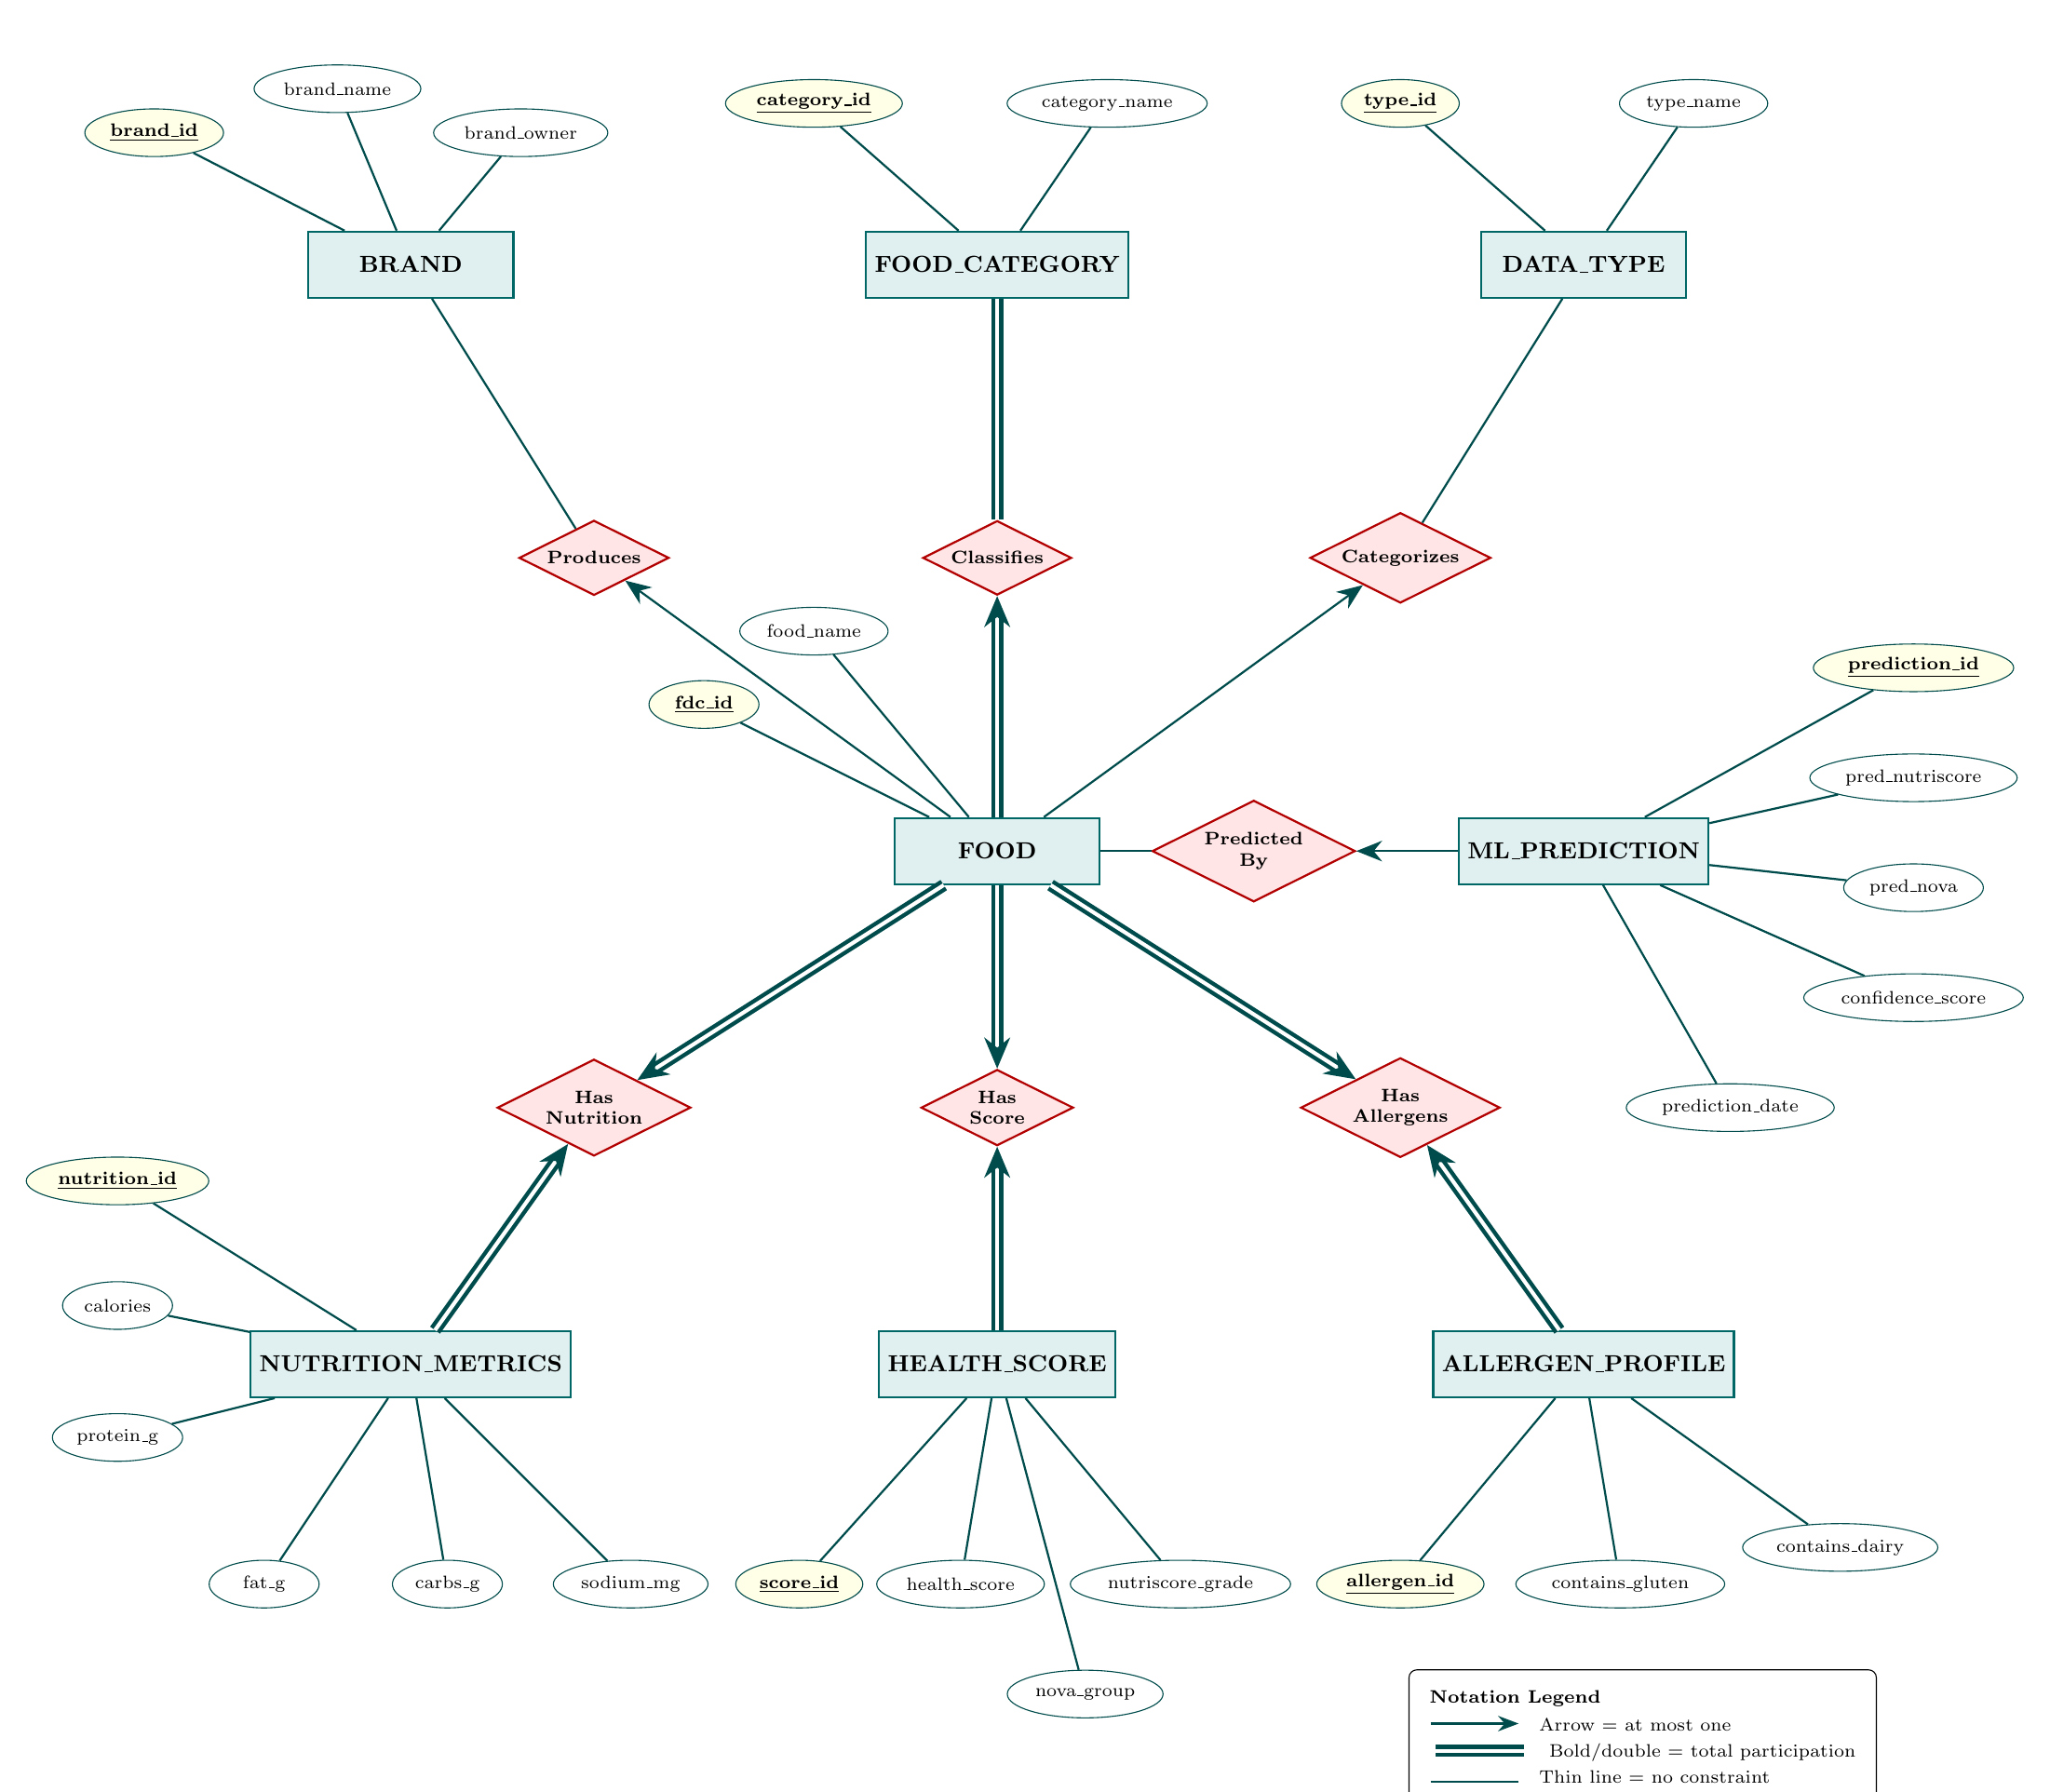
\begin{tikzpicture}[font=\small, node distance=3cm and 4cm]

\tikzset{
  entity/.style={draw=teal!80!black, thick, fill=teal!12,
                 minimum width=2.8cm, minimum height=0.9cm, align=center,
                 font=\small\bfseries},
  attr/.style={draw=teal!60!black, thin, fill=white,
               ellipse, minimum width=1.5cm, minimum height=0.65cm,
               align=center, font=\scriptsize, inner sep=2pt},
  keyattr/.style={draw=teal!60!black, thin, fill=yellow!10,
                  ellipse, minimum width=1.5cm, minimum height=0.65cm,
                  align=center, font=\scriptsize\bfseries, inner sep=2pt},
  rel/.style={draw=red!70!black, thick, fill=red!10,
              diamond, minimum width=1.8cm, minimum height=1cm,
              align=center, font=\scriptsize\bfseries, inner sep=2pt, aspect=2},
  % Chen's constraint lines:
  %   thin line        = no constraint (partial participation, many)
  %   arrow (->)       = at most one
  %   double/bold line = total participation
  rl/.style={thick, teal!60!black},
  arl/.style={thick, teal!60!black, -{Stealth[length=10pt, width=8pt]}},
  trl/.style={ultra thick, teal!60!black, double, double distance=1.5pt},
  tarl/.style={ultra thick, teal!60!black, double, double distance=1.5pt, -{Stealth[length=12pt, width=10pt]}},
}

% === ENTITIES ===
\node[entity] (brand) at (0, 0) {BRAND};
\node[entity] (fcat) at (8, 0) {FOOD\_CATEGORY};
\node[entity] (dtype) at (16, 0) {DATA\_TYPE};
\node[entity] (food) at (8, -8) {FOOD};
\node[entity] (nutr) at (0, -15) {NUTRITION\_METRICS};
\node[entity] (health) at (8, -15) {HEALTH\_SCORE};
\node[entity] (allerg) at (16, -15) {ALLERGEN\_PROFILE};
\node[entity] (mlpred) at (16, -8) {ML\_PREDICTION};

% === BRAND attrs ===
\node[keyattr] (a1) at (-3.5, 1.8) {\underline{brand\_id}};
\node[attr] (a2) at (-1, 2.4) {brand\_name};
\node[attr] (a3) at (1.5, 1.8) {brand\_owner};
\draw[rl] (brand)--(a1); \draw[rl] (brand)--(a2); \draw[rl] (brand)--(a3);

% === FOOD_CATEGORY attrs ===
\node[keyattr] (b1) at (5.5, 2.2) {\underline{category\_id}};
\node[attr] (b2) at (9.5, 2.2) {category\_name};
\draw[rl] (fcat)--(b1); \draw[rl] (fcat)--(b2);

% === DATA_TYPE attrs ===
\node[keyattr] (c1) at (13.5, 2.2) {\underline{type\_id}};
\node[attr] (c2) at (17.5, 2.2) {type\_name};
\draw[rl] (dtype)--(c1); \draw[rl] (dtype)--(c2);

% === FOOD attrs ===
\node[keyattr] (d1) at (4.0, -6.0) {\underline{fdc\_id}};
\node[attr] (d2) at (5.5, -5.0) {food\_name};
\draw[rl] (food)--(d1); \draw[rl] (food)--(d2);

% === NUTRITION attrs ===
\node[keyattr] (e1) at (-4.0, -12.5) {\underline{nutrition\_id}};
\node[attr] (e2) at (-4.0, -14.2) {calories};
\node[attr] (e3) at (-4.0, -16.0) {protein\_g};
\node[attr] (e4) at (-2.0, -18.0) {fat\_g};
\node[attr] (e5) at (0.5, -18.0) {carbs\_g};
\node[attr] (e6) at (3.0, -18.0) {sodium\_mg};
\draw[rl] (nutr)--(e1); \draw[rl] (nutr)--(e2); \draw[rl] (nutr)--(e3);
\draw[rl] (nutr)--(e4); \draw[rl] (nutr)--(e5); \draw[rl] (nutr)--(e6);

% === HEALTH_SCORE attrs ===
\node[keyattr] (f1) at (5.3, -18.0) {\underline{score\_id}};
\node[attr] (f2) at (7.5, -18.0) {health\_score};
\node[attr] (f3) at (10.5, -18.0) {nutriscore\_grade};
\node[attr] (f4) at (9.2, -19.5) {nova\_group};
\draw[rl] (health)--(f1); \draw[rl] (health)--(f2);
\draw[rl] (health)--(f3); \draw[rl] (health)--(f4);

% === ALLERGEN attrs ===
\node[keyattr] (g1) at (13.5, -18.0) {\underline{allergen\_id}};
\node[attr] (g2) at (16.5, -18.0) {contains\_gluten};
\node[attr] (g3) at (19.5, -17.5) {contains\_dairy};
\draw[rl] (allerg)--(g1); \draw[rl] (allerg)--(g2); \draw[rl] (allerg)--(g3);

% === ML_PREDICTION attrs ===
\node[keyattr] (h1) at (20.5, -5.5) {\underline{prediction\_id}};
\node[attr] (h2) at (20.5, -7.0) {pred\_nutriscore};
\node[attr] (h3) at (20.5, -8.5) {pred\_nova};
\node[attr] (h4) at (20.5, -10.0) {confidence\_score};
\node[attr] (h5) at (18.0, -11.5) {prediction\_date};
\draw[rl] (mlpred)--(h1); \draw[rl] (mlpred)--(h2);
\draw[rl] (mlpred)--(h3); \draw[rl] (mlpred)--(h4); \draw[rl] (mlpred)--(h5);

% === RELATIONSHIPS (Chen's constraint notation) ===
%   Arrow   = at most one  |  Double line = total  |  Thin line = no constraint

% BRAND --Produces-- FOOD  (1:N, partial-partial)
%   BRAND side: thin line (partial, no constraint → many foods)
%   FOOD side:  thin arrow toward diamond (partial, at most one brand)
\node[rel] (r1) at (2.5, -4) {Produces};
\draw[rl]  (brand) -- (r1);
\draw[arl] (food)  -- (r1);

% FOOD_CATEGORY --Classifies-- FOOD  (1:N, total-total)
%   CATEGORY side: double line (total, no constraint → many foods)
%   FOOD side:     double arrow (total, at most one category)
\node[rel] (r2) at (8, -4) {Classifies};
\draw[trl]  (fcat) -- (r2);
\draw[tarl] (food) -- (r2);

% DATA_TYPE --Categorizes-- FOOD  (1:N, partial-partial)
%   TYPE side: thin line (partial, no constraint → many foods)
%   FOOD side: thin arrow (partial, at most one type)
\node[rel] (r3) at (13.5, -4) {Categorizes};
\draw[rl]  (dtype) -- (r3);
\draw[arl] (food)  -- (r3);

% FOOD --Has Nutrition-- NUTRITION_METRICS  (1:1, total-total)
%   Both sides: double arrow (total, at most one)
\node[rel] (r4) at (2.5, -11.5) {Has\\Nutrition};
\draw[tarl] (food) -- (r4);
\draw[tarl] (nutr) -- (r4);

% FOOD --Has Score-- HEALTH_SCORE  (1:1, total-total)
\node[rel] (r5) at (8, -11.5) {Has\\Score};
\draw[tarl] (food)   -- (r5);
\draw[tarl] (health) -- (r5);

% FOOD --Has Allergens-- ALLERGEN_PROFILE  (1:1, total-total)
\node[rel] (r6) at (13.5, -11.5) {Has\\Allergens};
\draw[tarl] (food)   -- (r6);
\draw[tarl] (allerg) -- (r6);

% FOOD --Predicted By-- ML_PREDICTION  (1:N, partial-partial)
%   FOOD side: thin line (partial, no constraint → many predictions)
%   ML side:   thin arrow (partial, at most one food)
\node[rel] (r7) at (11.5, -8) {Predicted\\By};
\draw[rl]  (food)   -- (r7);
\draw[arl] (mlpred) -- (r7);

% === LEGEND ===
\node[draw, fill=white, rounded corners=3pt, inner sep=8pt,
      font=\scriptsize, align=left, anchor=south east] at (20, -21) {
  \textbf{Notation Legend}\\[3pt]
  \tikz\draw[thick, teal!60!black, -{Stealth[length=8pt, width=6pt]}] (0,0) -- (1.2,0); \; Arrow $=$ at most one\\[2pt]
  \tikz\draw[ultra thick, teal!60!black, double, double distance=1.5pt] (0,0) -- (1.2,0); \; Bold/double $=$ total participation\\[2pt]
  \tikz\draw[thick, teal!60!black] (0,0) -- (1.2,0); \; Thin line $=$ no constraint
};

\end{tikzpicture}%
}
\caption{NutriQuery 3NF ER Diagram -- Chen's Notation}
\label{fig:er}
\end{figure}

\subsection{Constraint Summary}
\begin{table}[H]\centering\small
\resizebox{\textwidth}{!}{%
\begin{tabular}{lcccc}
\toprule
\textbf{Relationship} & \textbf{Card.} & \textbf{Left Line} & \textbf{Right Line} & \textbf{Meaning} \\
\midrule
BRAND -- FOOD & 1:N & thin & arrow & Partial; each food $\leq$ 1 brand \\
FOOD\_CATEGORY -- FOOD & 1:N & double & double+arrow & Total; each food exactly 1 category \\
DATA\_TYPE -- FOOD & 1:N & thin & arrow & Partial; each food $\leq$ 1 type \\
FOOD -- NUTR. & 1:1 & double+arrow & double+arrow & Total both; exactly 1--1 \\
FOOD -- HEALTH & 1:1 & double+arrow & double+arrow & Total both; exactly 1--1 \\
FOOD -- ALLERG. & 1:1 & double+arrow & double+arrow & Total both; exactly 1--1 \\
FOOD -- ML\_PRED. & 1:N & thin & arrow & Partial; each pred. $\leq$ 1 food \\
\bottomrule
\end{tabular}%
}
\caption{Cardinality and participation constraints}
\end{table}

\subsection{Advanced Features}
Our domain does not require weak entities or ISA hierarchies. Every entity has its own strong primary key (either a natural USDA identifier or a surrogate \texttt{IDENTITY} key). There are no generalization/specialization hierarchies among food types that would warrant an ISA construct.

% ══════════════════════════════════════════════════════════════════════════════
\section{Part II: Relational Schema Translation}

Each strong entity becomes a relation. All relationships are either 1:1 or 1:N, so they are folded into the ``many'' (or dependent) side via a foreign key. No separate relationship tables are needed (no M:N relationships exist).

\subsection{Translated Relations}

\begin{sqlbox}[3NF Relational Schema]
\small
\begin{verbatim}
BRAND (
    brand_id    INT  IDENTITY  PRIMARY KEY,
    brand_name  VARCHAR(255)   NOT NULL,
    brand_owner VARCHAR(255)   NULL
)

FOOD_CATEGORY (
    category_id   INT  IDENTITY  PRIMARY KEY,
    category_name VARCHAR(255)   NOT NULL  UNIQUE
)

DATA_TYPE (
    type_id   INT  IDENTITY  PRIMARY KEY,
    type_name VARCHAR(100)   NOT NULL  UNIQUE
)

FOOD (
    fdc_id      INT           PRIMARY KEY,
    brand_id    INT           FK -> BRAND(brand_id)      NULL,
    category_id INT           FK -> FOOD_CATEGORY(category_id),
    type_id     INT           FK -> DATA_TYPE(type_id)   NULL,
    food_name   VARCHAR(500)  NOT NULL
)

NUTRITION_METRICS (
    nutrition_id INT  IDENTITY  PRIMARY KEY,
    fdc_id       INT  NOT NULL  UNIQUE  FK -> FOOD(fdc_id),
    calories     FLOAT NULL,
    protein_g    FLOAT NULL,
    fat_g        FLOAT NULL,
    carbs_g      FLOAT NULL,
    sodium_mg    FLOAT NULL
)

HEALTH_SCORE (
    score_id        INT  IDENTITY  PRIMARY KEY,
    fdc_id          INT  NOT NULL  UNIQUE  FK -> FOOD(fdc_id),
    health_score    FLOAT       NULL,
    nutriscore_grade VARCHAR(50) NULL,
    nova_group      INT         NULL
)

ALLERGEN_PROFILE (
    allergen_id     INT  IDENTITY  PRIMARY KEY,
    fdc_id          INT  NOT NULL  UNIQUE  FK -> FOOD(fdc_id),
    contains_gluten BIT  DEFAULT 0,
    contains_dairy  BIT  DEFAULT 0
)

ML_PREDICTION (
    prediction_id      INT  IDENTITY  PRIMARY KEY,
    fdc_id             INT  NOT NULL  FK -> FOOD(fdc_id),
    predicted_nutriscore VARCHAR(50) NULL,
    predicted_nova     INT          NULL,
    confidence_score   FLOAT        NULL,
    prediction_date    DATETIME     DEFAULT GETDATE()
)
\end{verbatim}
\end{sqlbox}

\subsection{Translation Rationale}
\begin{itemize}
  \item \textbf{1:N relationships} (Produces, Classifies, Categorizes, Predicted By): The foreign key is placed in the ``many'' side (\texttt{FOOD} or \texttt{ML\_PREDICTION}).
  \item \textbf{1:1 relationships} (Has Nutrition, Has Score, Has Allergens): The foreign key \texttt{fdc\_id} with a \texttt{UNIQUE} constraint is placed in the dependent entity, enforcing a strict one-to-one mapping.
  \item \textbf{No M:N tables needed}: All relationships are resolved with embedded foreign keys.
  \item \textbf{No weak entities or ISA hierarchies}: Not applicable to our domain.
\end{itemize}

% ══════════════════════════════════════════════════════════════════════════════
\section{Part III: Functional Dependencies (FDs)}
% ══════════════════════════════════════════════════════════════════════════════

Below we list all non-trivial functional dependencies for each relation, derived from the real-world semantics of the NutriQuery domain.

\textbf{Note on Partial and Transitive Dependencies:} Because our conceptual ER design translates directly into an optimal schema, the final relations presented here exhibit no partial dependencies (as all primary keys are single-column) and no transitive dependencies. However, to explicitly demonstrate our ability to identify and resolve them as per the assignment requirements, we analyze an unnormalized baseline schema containing transitive dependencies and perform a step-by-step reduction in \textbf{Part IV}.

\subsection{FDs per Relation}

\begin{fdbox}[Final 3NF/BCNF Dependencies]
\paragraph{BRAND}
\begin{align}
\texttt{brand\_id} &\to \texttt{brand\_name, brand\_owner} \label{fd:b1}
\end{align}

\paragraph{FOOD\_CATEGORY}
\begin{align}
\texttt{category\_id} &\to \texttt{category\_name} \\
\texttt{category\_name} &\to \texttt{category\_id} \quad \text{(UNIQUE constraint -- candidate key)}
\end{align}

\paragraph{DATA\_TYPE}
\begin{align}
\texttt{type\_id} &\to \texttt{type\_name} \\
\texttt{type\_name} &\to \texttt{type\_id} \quad \text{(UNIQUE constraint -- candidate key)}
\end{align}

\paragraph{FOOD}
\begin{align}
\texttt{fdc\_id} &\to \texttt{food\_name, brand\_id, category\_id, type\_id}
\end{align}

\paragraph{NUTRITION\_METRICS}
\begin{align}
\texttt{nutrition\_id} &\to \texttt{fdc\_id, calories, protein\_g, fat\_g,} \notag \\
                       &\quad\; \texttt{carbs\_g, sodium\_mg} \\
\texttt{fdc\_id} &\to \texttt{nutrition\_id, calories, protein\_g, fat\_g,} \notag \\
                 &\quad\; \texttt{carbs\_g, sodium\_mg}
\end{align}

\paragraph{HEALTH\_SCORE}
\begin{align}
\texttt{score\_id} &\to \texttt{fdc\_id, health\_score, nutriscore\_grade,} \notag \\
                   &\quad\; \texttt{nova\_group} \\
\texttt{fdc\_id} &\to \texttt{score\_id, health\_score, nutriscore\_grade,} \notag \\
                 &\quad\; \texttt{nova\_group}
\end{align}

\paragraph{ALLERGEN\_PROFILE}
\begin{align}
\texttt{allergen\_id} &\to \texttt{fdc\_id, contains\_gluten, contains\_dairy} \\
\texttt{fdc\_id} &\to \texttt{allergen\_id, contains\_gluten, contains\_dairy}
\end{align}

\paragraph{ML\_PREDICTION}
\begin{align}
\texttt{prediction\_id} &\to \texttt{fdc\_id, predicted\_nutriscore, predicted\_nova,} \notag \\
                        &\quad\; \texttt{confidence\_score, prediction\_date}
\end{align}
Note: \texttt{fdc\_id} is \emph{not} a candidate key in ML\_PREDICTION since one food can have multiple predictions over time.
\end{fdbox}

% ══════════════════════════════════════════════════════════════════════════════
\section{Part IV: Normalization}
% ══════════════════════════════════════════════════════════════════════════════

To mathematically ensure our final schema (presented in Parts I-III) is free from anomalies, we evaluate the database design against functional dependencies using the standard normalization process. We start from an unnormalized baseline (our prior HW2 schema) and systematically derive the 3NF/BCNF relations.

\subsection{Initial Schema (HW2 Baseline)}
The prior version of our database contained the following 5 tables, which suffered from transitive dependencies and grouped multiple concerns into single relations:

\begin{sqlbox}[Unnormalized HW2 Schema]
\small
\begin{verbatim}
Brands(brand_id, brand_name, brand_owner, ecoscore_grade)
Foods(fdc_id, brand_id, food_name, data_type, food_category)
Nutrition_Metrics(nutrition_id, fdc_id, calories, protein_g,
                  fat_g, carbs_g, sodium_mg)
Health_and_Allergens(profile_id, fdc_id, contains_gluten,
                     contains_dairy, health_score,
                     nutriscore_grade, nova_group)
ML_Predictions(prediction_id, fdc_id, predicted_nutriscore,
               predicted_nova, confidence_score, prediction_date)
\end{verbatim}
\end{sqlbox}

\subsection{Before-Normalization Functional Dependencies}
Based on the unnormalized schema and domain semantics, we identify the following initial functional dependencies (FDs) representing the business rules \emph{before} normalization:

\begin{fdbox}[Initial Functional Dependencies]
\begin{enumerate}[label=\textbf{FD\arabic*:}]
    \item \texttt{fdc\_id} $\to$ \texttt{food\_name}, \texttt{brand\_id}, \texttt{data\_type}, \texttt{food\_category}
    \item \texttt{brand\_id} $\to$ \texttt{brand\_name}, \texttt{brand\_owner}, \texttt{ecoscore\_grade} (Anomalous dependency: ecoscore actually depends on the product \texttt{fdc\_id}, not the brand).
    \item \texttt{nutrition\_id} $\to$ \texttt{fdc\_id}, \texttt{calories}, \texttt{protein\_g}, \texttt{fat\_g}, \texttt{carbs\_g}, \texttt{sodium\_mg}
    \item \texttt{profile\_id} $\to$ \texttt{fdc\_id}, \texttt{contains\_gluten}, \texttt{contains\_dairy}, \\ \texttt{health\_score}, \texttt{nutriscore\_grade}, \texttt{nova\_group}
    \item \texttt{prediction\_id} $\to$ \texttt{fdc\_id}, \texttt{predicted\_nutriscore}, \texttt{predicted\_nova}, \\ \texttt{confidence\_score}, \texttt{prediction\_date}
\end{enumerate}
\end{fdbox}

\subsection{Step 1: First Normal Form (1NF)}
\textbf{Requirement:} All attributes must be atomic (single-valued); no repeating groups. \\
\textbf{Analysis:} The initial schema already satisfies 1NF because every column stores a single scalar value (INT, FLOAT, VARCHAR, BIT, DATETIME), and there are no multi-valued or array-type attributes. \\
\textbf{Result:} No changes needed. $\checkmark$ \textbf{1NF satisfied.}

\subsection{Step 2: Second Normal Form (2NF)}
\textbf{Requirement:} Must be in 1NF, and every non-key attribute must be fully functionally dependent on the \emph{entire} primary key (no partial dependencies). \\
\textbf{Analysis:} Every table in the original schema uses a \textbf{single-column primary key} (\texttt{brand\_id}, \texttt{fdc\_id}, \texttt{nutrition\_id}, \texttt{profile\_id}, \texttt{prediction\_id}). Partial dependencies can only arise with composite keys. \\
\textbf{Result:} No changes needed. $\checkmark$ \textbf{2NF satisfied.}

\subsection{Step 3: Third Normal Form (3NF) \& BCNF}
\textbf{Requirement:} Must be in 2NF, and no non-key attribute may transitively depend on the primary key (i.e., $X \to Y \to Z$ where $Y$ is not a candidate key). We evaluate the baseline tables against our FDs to eliminate update, insertion, and deletion anomalies.

\textbf{Analysis -- Four major violations found and fixed:}

\subsubsection*{Violation 1: \texttt{ecoscore\_grade} in \texttt{Brands}}
\texttt{ecoscore\_grade} is a product-level environmental score, not a brand-level property. Different products from the same brand have different eco-scores. This violates FD semantics. \\
\textbf{Fix:} Remove \texttt{ecoscore\_grade} from \texttt{BRAND}.

\subsubsection*{Violation 2: \texttt{food\_category} in \texttt{Foods}}
\texttt{food\_category} is a repeating VARCHAR string. Renaming a category requires updating every matching row $\Rightarrow$ \textbf{update anomaly}. \\
\textbf{Fix:} Extract to a new \texttt{FOOD\_CATEGORY(category\_id, category\_name)} table. Replace the VARCHAR column with an FK \texttt{category\_id} in \texttt{FOOD}.

\subsubsection*{Violation 3: \texttt{data\_type} in \texttt{Foods}}
Identical issue to \texttt{food\_category} -- a repeating string like ``SR Legacy. \\
\textbf{Fix:} Extract to \texttt{DATA\_TYPE(type\_id, type\_name)}. Replace with FK \texttt{type\_id} in \texttt{FOOD}.

\subsubsection*{Violation 4: Mixed concerns in \texttt{Health\_and\_Allergens}}
This table groups two functionally independent attribute sets: Scoring (\texttt{health\_score}) and Allergens (\texttt{contains\_gluten}). Allergen status does not determine health scores. Grouping them violates single-concern design and creates insertion/deletion anomalies. \\
\textbf{Fix:} Decompose into:
\begin{itemize}
  \item \texttt{HEALTH\_SCORE(score\_id, fdc\_id,} \\ \texttt{health\_score, nutriscore\_grade, nova\_group)}
  \item \texttt{ALLERGEN\_PROFILE(allergen\_id,} \\ \texttt{fdc\_id, contains\_gluten, contains\_dairy)}
\end{itemize}

\textbf{Result:} After these extractions, the original schema grows from 5 to 8 tables. Every determinant in the resulting 8 tables is a candidate key, meaning the schema fully satisfies \textbf{Boyce-Codd Normal Form (BCNF)}.

\vspace{1em}
\hrule
\vspace{1em}
{\sloppy \textit{This step-by-step standard normalization process mathematically proves the integrity of the final 3NF schema modeled and translated in the preceding sections.} \par}


\end{document}
